\section{Auditing the injector}\label{sec:injector}

A fault-injection result is only as good as the record of what was
injected. emufi keeps a ring of every flip: sequence number, time,
sector, operation, byte offset in the bio segment, bit, value before and
after. Matching that ring against the corrections the kernel reported
exposed a defect in the record, which this section explains, measures
and works around. emufi is part of the sealed image and was not changed
for this report.

\subsection{Two hooks, one of them a bio early}

emufi 0.8.1 acts on read completions through two kprobes
(\cref{fig:hooks}). The first, on \texttt{blk\_update\_request}, runs
while the bio iterator is intact: it logs the bio's start sector and
flips a bit in its first segment. The block layer then calls
\texttt{bio\_advance} and \texttt{bio\_endio}, where the second kprobe
runs. emufi assumes that by then the iterator has been consumed, the
start sector advanced past the transfer, and recovers the start by
subtracting the transfer size. In Linux 7.3-rc5, \texttt{bio\_advance}
of a complete transfer only zeroes the size and leaves the start sector
where it was (\texttt{include/linux/bio.h} at
\texttt{72d3fcf8}~\cite{linux73rc5}). The second hook therefore logs,
and filters on, the span one bio \emph{before} the bio it flips.

Three consequences follow. A \bfs read bio, one 4\,KiB block, can take
two flips, one per hook, each drawn with probability $p$. The second
flip is logged eight sectors early. And the second hook attacks the
block that follows each target block: in run 4 that put the indirect
block of the target file, which follows its twelfth data block, within
reach although the range list excluded it. A filesystem that reads the
file in multi-block bios is touched by the first hook only, the shifted
span falling before the file: ext4 here, one hook invocation per attack.

\begin{figure}[t]
\centering
\begin{tikzpicture}[font=\scriptsize,node distance=3.2mm,
  box/.style={draw,rounded corners=1pt,align=center,inner sep=2pt,minimum height=6mm,text width=21mm},
  hook/.style={box,fill=orange!20}]
  \node[box] (dev) {device completes\\read of block $b$\\(sector $s$)};
  \node[hook,right=of dev] (rq) {\texttt{blk\_update\_}\\\texttt{request}\\hook 1: logs $s$,\\flips block $b$};
  \node[box,right=of rq] (adv) {\texttt{bio\_advance}:\\size $\to 0$,\\sector stays $s$};
  \node[hook,below=4mm of adv] (ep) {\texttt{bio\_endio}\\hook 2: logs $s-8$,\\flips block $b$};
  \node[box,left=of ep,fill=red!8] (rec) {ring: $(s)$ then $(s-8)$,\\at most \dtPairMaxMicro\,$\mu$s apart};
  \draw[-{Stealth}] (dev) -- (rq);
  \draw[-{Stealth}] (rq) -- (adv);
  \draw[-{Stealth}] (adv) -- (ep);
  \draw[-{Stealth}] (ep) -- (rec);
\end{tikzpicture}
\caption{The two read hooks of emufi 0.8.1 on Linux 7.3-rc5. Both flip
the block that was read; the second logs it eight sectors (one 4\,KiB
block) early.}
\label{fig:hooks}
\end{figure}

\subsection{Recovering the hook of every flip}

In ring order, an entry at sector $s$ followed within
\dtPairMaxMicro\,$\mu$s by
one at $s-8$ is the pair of one bio, both flips in block $s/8$. At
$p=10^{6}$\,ppm both hooks fire whenever the filter admits them, so an
entry left alone has one explanation: the first hook of a bio whose
shifted span the filter refused (the first target block), or the second
hook of a bio whose own block the filter refused (the block after a
target block). Below $10^{6}$\,ppm either hook may have drawn alone, and
a lone entry is ambiguous between its logged block and the next.

\subsection{Checking the reconstruction}

The reconstruction is checked three ways, all by the extraction script
before any table is written.
\begin{itemize}
\item \emph{Timing.} Over the three $10^{6}$\,ppm attacks, the two
  entries of a pair are at most \dtPairMaxMicro\,$\mu$s apart; two
  consecutive entries that are not a pair are at least
  \dtOtherMinMilli\,ms apart. No interval falls between.
\item \emph{Completeness.} At $10^{6}$\,ppm every flip is attributed
  (\ambiguousHigh{} ambiguous).
\item \emph{The kernel's account.} \bfs logs each correction with the
  inode, the logical block, the codeword and the number of symbols
  corrected, rate-limited to the first ten lines of an attack. All
  \kernLines{} lines are explained by flips at the reconstructed block
  and codeword, or, for an ambiguous flip, at its logged block or the
  next; none is left over. In run 3 at $10^{6}$\,ppm one decode
  corrected two symbols in one codeword: the two flips of one bio, the
  first in that codeword's parity, the second in its data.
\end{itemize}

\Cref{tab:rs} summarises the six \bfs attacks that received flips. With
one bit per hook, a decode sees at most two erroneous symbols in a
codeword; the kernel reported at most \kernMaxPerDecode{}. Taking the
union over a whole attack, which overstates what any decode saw, no
codeword was hit in more than \unionMax{} distinct symbols. The budget
is eight. \Cref{fig:rsmap} shows where the flips fell.

\begin{table*}[t]
\centering
\caption{\bfs attacks with flips: flips received, target filter in
effect, hook pairs and lone entries, kernel lines (all explained), most
symbols corrected in one decode (kernel), most distinct symbols hit in
one codeword over the attack, counting only flips whose block is known
(none at $10^{5}$\,ppm in run 4, where every flip was alone).}
\label{tab:rs}
\footnotesize
\setlength{\tabcolsep}{3pt}
\begin{tabular}{@{}lrrlrrrrr@{}}
\toprule
run & ppm & flips & target & pairs & single & k-lines & dec & union \\
\midrule
2 & 100\,000 & 20 & interval & 2 & 16 & 10 & 1 & 1 \\
2 & 1\,000\,000 & 265 & interval & 132 & 1 & 10 & 1 & 2 \\
3 & 100\,000 & 22 & interval & 1 & 20 & 10 & 1 & 1 \\
3 & 1\,000\,000 & 265 & interval & 132 & 1 & 10 & 2 & 3 \\
4 & 100\,000 & 33 & list & 0 & 33 & 10 & 1 & 0 \\
4 & 1\,000\,000 & 262 & list & 129 & 4 & 10 & 1 & 3 \\
\bottomrule
\end{tabular}

\end{table*}

\begin{figure*}[t]
\centering
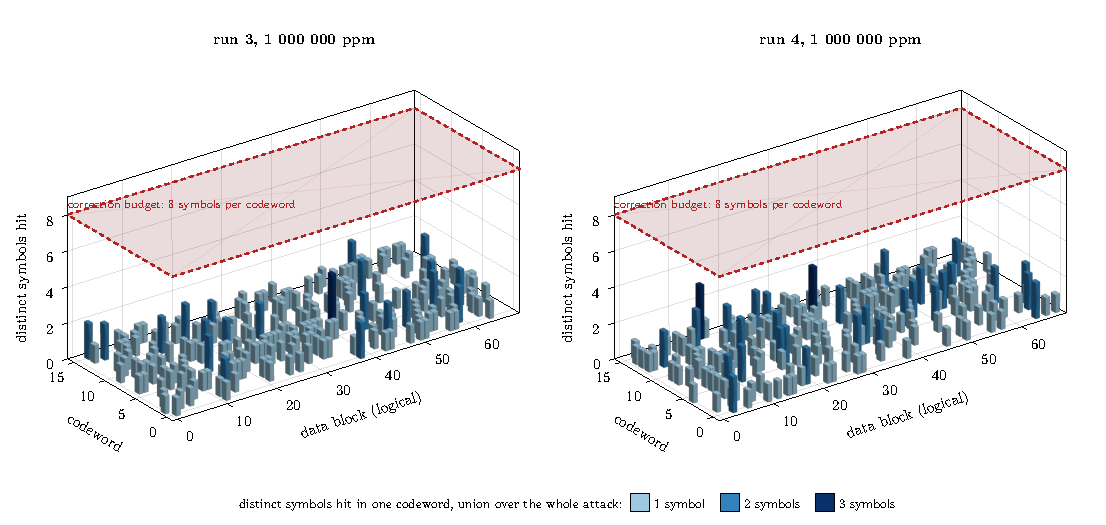
\includegraphics[width=\textwidth]{figures/rsmap-3d.pdf}
\caption{\bfs at $10^{6}$\,ppm, runs 3 and 4: for each data block and
codeword, the number of distinct symbols hit over the whole attack
(flips of known block only). The plane marks the eight symbols one
codeword corrects; no column exceeds \unionMax{}.}
\label{fig:rsmap}
\end{figure*}
